\section{Results}
\label{sec:results}

We report closure rates across the 20-cell DOE on the 150-function core dataset, comprising 5{,}890 measurement rows across the 20 cells $\times$ 3 paths, with mono cells at $n = 150$ samples/cell and hetero/null cells at $n = 75$ (H1, the pre-registered hetero champion, was re-swept during the human-evaluation extension, adding 41 rows above the $5{,}850$-row nominal schema; H7 lost one row to a parse failure). Results are organized by research question. Reported per-cell aggregates are either the metric mean $\bar{Y}_{a, p}$ (Eq.~\ref{eq:metric_mean}, in Table~\ref{tab:closure_rate_matrix} and Fig.~\ref{fig:closure_heatmap}) or the strict-AND valid-closure fraction $V_{a, p}$ (Eq.~\ref{eq:valid_closure_frac}, everywhere else), and every subsection identifies which. The strict-AND policy uses default thresholds $\tau_1 = \tau_2 = \tau_3 = 0$ and $\rho = 3$; the sensitivity analysis (Section~\ref{sec:experiment_setup_sensitivity}) confirms every headline finding survives alternative threshold choices.

\subsection{Metric means per cell and path}
\label{sec:results_closure_matrix}

Table~\ref{tab:closure_rate_matrix} and Fig.~\ref{fig:closure_heatmap} present the per-cell metric mean $\bar{Y}_{a, p}$ (Eq.~\ref{eq:metric_mean}) for every cell $\times$ path combination. This subsection reports metric means; the strict-AND valid-closure fraction $V_{a, p}$ is reported per-cell in Sections~\ref{sec:results_stage_attribution} and~\ref{sec:results_contamination} and in Appendix~\ref{sec:human_eval_strict_and}. Three high-level patterns emerge.

\needspace{22\baselineskip}

\noindent
\centering
\begin{tabular}{@{}lccc@{}}
\toprule
Cell & Path 1 & Path 2 & Path 3 \\
\midrule
M1   & 0.577~(75) & 0.367~(45) & 0.245~(61) \\
M2   & 0.769~(63) & 0.547~(71) & 0.185~(81) \\
M3   & \textbf{0.900}~(100) & 0.647~(90) & 0.208~(105) \\
M4   & 0.856~(116) & 0.647~(87) & \textbf{0.282}~(109) \\
M5   & 0.781~(98) & 0.533~(69) & 0.261~(80) \\
M6   & 0.862~(108) & 0.647~(86) & 0.219~(100) \\
\midrule
H1   & 0.854~(64) & \textbf{0.674}~(57) & 0.194~(56) \\
H2   & 0.862~(35) & 0.613~(40) & 0.185~(40) \\
H3   & 0.787~(50) & 0.627~(42) & 0.174~(29) \\
H4   & 0.862~(60) & 0.453~(30) & 0.199~(50) \\
H5   & 0.811~(50) & 0.667~(47) & 0.218~(37) \\
H6   & 0.882~(53) & 0.600~(41) & 0.184~(49) \\
H7   & 0.872~(57) & 0.600~(42) & 0.200~(53) \\
H8   & 0.846~(53) & 0.600~(43) & 0.260~(54) \\
H9   & 0.881~(54) & 0.627~(46) & 0.202~(55) \\
H10  & 0.764~(22) & 0.613~(42) & 0.248~(47) \\
H11  & 0.872~(61) & 0.653~(46) & 0.173~(50) \\
\midrule
N1   & 0.429~(23) & 0.120~(7) & 0.174~(20) \\
N2   & --- & 0.667~(47) & 0.000~(0) \\
N3   & --- & 0.000~(0) & 0.000~(0) \\
\bottomrule
\end{tabular}

\captionof{table}{Metric mean $\bar{Y}_{a, p}$ per cell $\times$ path (Eq.~\ref{eq:metric_mean}); the parenthetical is the strict-AND valid-closure count $n_{\text{valid}} = |\{r : Y_r > 0 \wedge J_r \geq 3\}|$, from which the valid-closure fraction $V_{a, p} = n_{\text{valid}} / N$ can be computed ($N = 150$ for mono; $N = 75$ for hetero and null; H1 has $N = 89$ on Paths 1 and 2 and $N = 88$ on Path 3 after the human-evaluation re-sweep). Metric $Y$: kill rate (Path~1), reference-test pass rate (Path~2), rescaled BERTScore F1 (Path~3). \textbf{Bold} marks the highest $\bar{Y}$ per path across non-null cells. N2 and N3 rows carry \texttt{---} for paths whose operative stage was ablated by construction (spec-ablation for N2, test-ablation for N3).}
\label{tab:closure_rate_matrix}

\medskip


\clearpage
\needspace{0.75\textheight}% fig2 is portrait (aspect 1.22) — needs ~70%% of textheight even at 0.75 linewidth
\noindent
\centering
\includegraphics[width=0.75\linewidth]{../plots/output/fig2_closure_heatmap.png}

\captionof{figure}{Metric mean $\bar{Y}_{a, p}$ per cell $\times$ path (heatmap; Eq.~\ref{eq:metric_mean}). Cell strata are (top to bottom) mono (M1--M6), hetero (H1--H11), and null (N1--N3). Values are raw per-cell means of the automated closure metric before the strict-AND validity policy is applied; the strict-AND valid-closure fraction $V_{a, p}$ is shown per cell in Table~\ref{tab:per_stage_bottleneck} and Fig.~\ref{fig:stage_contribution}.}
\label{fig:closure_heatmap}

\medskip

First, Path~1 (mutation kill rate) closure rates cluster in the $[0.7, 0.9]$ range for all non-null cells except M1, with a mean per-cell $\bar{Y}$ of $0.826$ across the 17 non-null cells. The strongest mono baseline is M3 (qwen3.6:27B, all stages) at $0.900$; the strongest hetero cell is H6 (phi-4/qwen3.6/phi-4) at $0.882$. The single mono failure is M1 (llama3.2:3B mono) at $0.577$.

Second, Path~2 (reference test pass rate) closure rates are systematically lower than Path~1, averaging $0.595$ across the 17 non-null cells. This reflects the harder nature of the code-synthesis task: passing the reference tests requires reconstructing the function's behavior exactly rather than merely covering it. Notably, the spec-stage-ablated null cell N2 (Path~2 closure rate $= 0.667$) ties or exceeds every mono baseline (M1 $= 0.367$, M2 $= 0.547$, others $\in [0.533, 0.647]$). We return to the implications of this in Section~\ref{sec:discussion_rq3}.

Third, Path~3 (BERTScore) closure rates are uniformly low, averaging $0.214$ across the 17 non-null cells, and vary in a compressed range $[0.17, 0.28]$. This is an artifact of BERTScore's rescaled value distribution on our data --- the natural distribution of BERTScore F1 values between original and reconstructed docstrings clusters in $[-0.1, 0.5]$. The compressed range does not indicate poor pipeline performance; Section~\ref{sec:discussion_rq2} shows that judge equivalence ratings on the same rows tell an entirely different story.

\subsection{Mono versus heterogeneous cells}
\label{sec:results_mono_vs_hetero}

\needspace{18\baselineskip}

\noindent
\centering
\includegraphics[width=0.90\linewidth]{../plots/output/fig3_mono_vs_hetero.png}

\captionof{figure}{Distribution of Path~1 closure rates across strata (mono, hetero, null). Each violin summarises the per-cell mean closure rates within a stratum.}
\label{fig:mono_vs_hetero}

\medskip

Fig.~\ref{fig:mono_vs_hetero} presents the per-strand distribution of closure rates on Path~1. The distributions overlap substantially: the median hetero cell ($0.862$) is competitive with the median mono cell ($0.819$), but the ceiling of each strand differs. The best mono cell (M3, kill rate $= 0.900$) exceeds the median hetero cell but not the best hetero cell (H6, $0.882$).

\begin{table}[!htbp]
\centering
\caption{Type-III ANOVA on closure metric (response) $\sim$ C(cell) + C(sample). Sums of squares are Type-III (each effect tested with all other terms in the model).}
\label{tab:anova}
\begin{tabular}{@{}lrrrrr@{}}
\toprule
Factor & Sum Sq & df & F & p & partial $\eta^2$ \\
\midrule
Intercept & 21.44 & 1 & 143.49 & $<0.001$ & 0.028 \\
C(cell_id) & 34.53 & 18 & 12.84 & $<0.001$ & 0.045 \\
C(sample_idx) & 148.00 & 149 & 6.65 & $<0.001$ & 0.168 \\
Residual & 732.69 & 4903 & --- & --- & --- \\
\bottomrule
\end{tabular}
\end{table}


To test whether cell-mean differences are statistically significant, we fit the ANOVA model of Eq.~\ref{eq:anova}; Table~\ref{tab:anova} presents the fitted terms. Cell is a significant predictor of closure rate under Type-III sums of squares ($F(18, 4903) = 12.84$, $p < 0.001$, partial $\eta^2 = 0.045$) after adjusting for per-sample difficulty. Tukey's HSD (Eq.~\ref{eq:tukey}), which controls family-wise error at $\alpha = 0.05$ over the $\binom{20}{2} = 190$ pairwise cell comparisons via the studentized-range distribution, identifies 35 pairs significant at $p_{\textsf{adj}} < 0.05$ and 33 significant at $p_{\textsf{adj}} < 0.01$ (Table~\ref{tab:tukey_significant}). The strongest single contrasts are:

\begin{table}[t]
\centering
\caption{Tukey HSD post-hoc — significant pairs at $\alpha = 0.05$, top 25 by $p_{\text{adj}}$. Bonferroni-corrected across the full 190-pair family.}
\label{tab:tukey}
\begin{tabular}{@{}lcccc@{}}
\toprule
Cell A & Cell B & $\Delta$ mean & $p_{\text{adj}}$ & Sig \\
\midrule
H1 & H4 & -0.253 & $<0.001$ & *** \\
H9 & M1 & -0.316 & $<0.001$ & *** \\
H8 & N3 & -0.363 & $<0.001$ & *** \\
H8 & N2 & -0.41 & $<0.001$ & *** \\
H8 & N1 & -0.571 & $<0.001$ & *** \\
H8 & M1 & -0.265 & $<0.001$ & *** \\
H7 & N3 & -0.264 & $<0.001$ & *** \\
H7 & N2 & -0.311 & $<0.001$ & *** \\
H7 & N1 & -0.472 & $<0.001$ & *** \\
H7 & M6 & 0.158 & $<0.001$ & *** \\
H7 & M4 & 0.106 & $<0.001$ & *** \\
H7 & M3 & 0.13 & $<0.001$ & *** \\
H9 & M5 & -0.13 & $<0.001$ & *** \\
H7 & M1 & -0.166 & $<0.001$ & *** \\
H6 & N3 & -0.333 & $<0.001$ & *** \\
H6 & N2 & -0.38 & $<0.001$ & *** \\
H6 & N1 & -0.54 & $<0.001$ & *** \\
H6 & M1 & -0.234 & $<0.001$ & *** \\
H5 & N3 & -0.213 & $<0.001$ & *** \\
H5 & N2 & -0.261 & $<0.001$ & *** \\
H5 & N1 & -0.421 & $<0.001$ & *** \\
H5 & M6 & 0.209 & $<0.001$ & *** \\
N1 & N2 & 0.16 & $<0.001$ & *** \\
H5 & M4 & 0.157 & $<0.001$ & *** \\
H5 & M3 & 0.18 & $<0.001$ & *** \\
\bottomrule
\end{tabular}
\end{table}


\begin{itemize}
  \item H1 vs.\ M1: $\Delta = -0.182$ ($p_{\textsf{adj}} < 0.001$) --- phi-4 in the spec stage plus qwen-coder in test/code stages substantially outperforms llama3.2 mono.
  \item H4 vs.\ N1: $\Delta = -0.262$ ($p_{\textsf{adj}} < 0.001$) --- every hetero cell beats the word-shuffled control by $> 0.25$, confirming that hetero closure signal is not a metric artifact.
  \item M1 vs.\ N2: $\Delta = +0.282$ ($p_{\textsf{adj}} < 0.001$) --- the spec-stage-ablated null cell N2 beats M1 mono; skipping the docstring stage and reusing the ground-truth docstring works better than generating a weak docstring in the first place.
\end{itemize}

The strongest non-directional finding is that the M3 mono ceiling and the best hetero cells cluster within $0.05$ of each other on Path~1. Section~\ref{sec:discussion_rq1} develops the interpretation that hetero pipelines \emph{match} rather than \emph{dominate} the strongest mono baseline on aggregate closure rate, and the more interesting stage-attribution structure emerges in the per-operator decomposition (Section~\ref{sec:results_per_operator}).

\subsection{Per-stage bottleneck attribution}
\label{sec:results_stage_attribution}

The bottleneck-attribution table (Table~\ref{tab:per_stage_bottleneck}) is computed on the metric mean $\bar{Y}_{a, p}$ (Eq.~\ref{eq:metric_mean}), consistent with Table~\ref{tab:closure_rate_matrix}; the stage-contribution figure (Fig.~\ref{fig:stage_contribution}) at the end of this subsection instead uses the strict-AND valid-closure fraction $V_{a, p}$ (Eq.~\ref{eq:valid_closure_frac}), so its numeric values differ from the table's. Each hetero cell composes three models $(m_{\textsf{spec}}, m_{\textsf{test}}, m_{\textsf{code}})$.

\begin{table}[t]
\centering
\caption{Per-stage bottleneck decomposition. For each hetero cell + path, the bottleneck stage is the one whose mono-cell mean is lowest. $\Delta$ to bottleneck = hetero\_mean $-$ mono(bottleneck) — positive means the hetero pipeline outperformed the bottleneck stage alone.}
\label{tab:bottleneck}
\begin{tabular}{@{}lccccccc@{}}
\toprule
Hetero & Path & Hetero mean & Mono(L\_spec) & Mono(L\_test) & Mono(L\_code) & Bottleneck stage & $\Delta$ to bottleneck \\
\midrule
H1 & 1 & 0.854 & 0.769 & 0.862 & 0.862 & spec & 0.085 \\
H1 & 2 & 0.674 & 0.547 & 0.647 & 0.647 & spec & 0.127 \\
H1 & 3 & 0.194 & 0.185 & 0.219 & 0.219 & spec & 0.009 \\
H2 & 1 & 0.862 & 0.9 & 0.769 & 0.862 & test & 0.093 \\
H2 & 2 & 0.613 & 0.647 & 0.547 & 0.647 & test & 0.067 \\
H2 & 3 & 0.185 & 0.208 & 0.185 & 0.219 & test & 0.0 \\
H3 & 1 & 0.787 & 0.856 & 0.781 & 0.862 & test & 0.006 \\
H3 & 2 & 0.671 & 0.647 & 0.533 & 0.647 & test & 0.138 \\
H3 & 3 & 0.221 & 0.282 & 0.261 & 0.219 & code & 0.001 \\
H4 & 1 & 0.862 & 0.862 & 0.862 & 0.577 & code & 0.285 \\
H4 & 2 & 0.453 & 0.647 & 0.647 & 0.367 & code & 0.087 \\
H4 & 3 & 0.199 & 0.219 & 0.219 & 0.245 & spec & -0.021 \\
H5 & 1 & 0.811 & 0.577 & 0.862 & 0.862 & spec & 0.234 \\
H5 & 2 & 0.667 & 0.367 & 0.647 & 0.647 & spec & 0.3 \\
H5 & 3 & 0.218 & 0.245 & 0.219 & 0.219 & test & -0.002 \\
H6 & 1 & 0.882 & 0.769 & 0.9 & 0.769 & spec & 0.113 \\
H6 & 2 & 0.6 & 0.547 & 0.647 & 0.547 & spec & 0.053 \\
H6 & 3 & 0.184 & 0.185 & 0.208 & 0.185 & spec & -0.001 \\
H7 & 1 & 0.872 & 0.862 & 0.9 & 0.769 & code & 0.103 \\
H7 & 2 & 0.6 & 0.647 & 0.647 & 0.547 & code & 0.053 \\
H7 & 3 & 0.2 & 0.219 & 0.208 & 0.185 & code & 0.015 \\
H8 & 1 & 0.846 & 0.856 & 0.862 & 0.781 & code & 0.065 \\
H8 & 2 & 0.6 & 0.647 & 0.647 & 0.533 & code & 0.067 \\
H8 & 3 & 0.26 & 0.282 & 0.219 & 0.261 & test & 0.04 \\
H9 & 1 & 0.881 & 0.862 & 0.9 & 0.862 & spec & 0.019 \\
H9 & 2 & 0.627 & 0.647 & 0.647 & 0.647 & spec & -0.02 \\
H9 & 3 & 0.202 & 0.219 & 0.208 & 0.219 & test & -0.006 \\
H10 & 1 & 0.764 & 0.781 & 0.769 & 0.862 & test & -0.005 \\
H10 & 2 & 0.613 & 0.533 & 0.547 & 0.647 & spec & 0.08 \\
H10 & 3 & 0.248 & 0.261 & 0.185 & 0.219 & test & 0.062 \\
H11 & 1 & 0.872 & 0.769 & 0.856 & 0.862 & spec & 0.103 \\
H11 & 2 & 0.653 & 0.547 & 0.647 & 0.647 & spec & 0.107 \\
H11 & 3 & 0.173 & 0.185 & 0.282 & 0.219 & spec & -0.012 \\
\bottomrule
\end{tabular}
\end{table}


Table~\ref{tab:per_stage_bottleneck} attributes each hetero cell's metric mean to the mono cell whose model appears at the same slot: for hetero cell $a$ and stage $s$, the \emph{stage baseline} $\hat{Y}_{a,s}$ is the metric mean of the mono cell using $a(s)$ at all stages. The \emph{bottleneck stage} is the stage whose baseline is the lowest, and $\Delta_a = \bar{Y}_a - \min_s \hat{Y}_{a,s}$ is the improvement from specializing the other two stages.

Across the 11 hetero cells, spec-stage attribution accounts for 15 of the 33 (cell $\times$ path) triples; test-stage 10; code-stage 8. The most striking single-stage attributions are:

\begin{itemize}
  \item \textbf{H4 code attribution, $\Delta = 0.285$ (Path~1)} --- qwen-coder at $L_{\textsf{spec}}$ and $L_{\textsf{test}}$, llama3.2 at $L_{\textsf{code}}$. Even the ``cheap drafter at the code stage'' composition recovers $28$ percentage points of kill rate over the llama3.2 mono baseline, suggesting that spec and test quality can compensate substantially for weak synthesis.
  \item \textbf{H5 spec attribution, $\Delta = 0.234$ (Path~1)} --- llama3.2 at $L_{\textsf{spec}}$, qwen-coder at $L_{\textsf{test}}$ and $L_{\textsf{code}}$. Substituting stronger models at test and code stages recovers $23$ percentage points of kill rate that llama3.2 mono cannot achieve alone; the same composition recovers $\Delta = 0.300$ on Path~2.
\end{itemize}

\clearpage
\needspace{0.55\textheight}% fig10 stage-contribution follows the tall per-stage-bottleneck table
\noindent
\centering
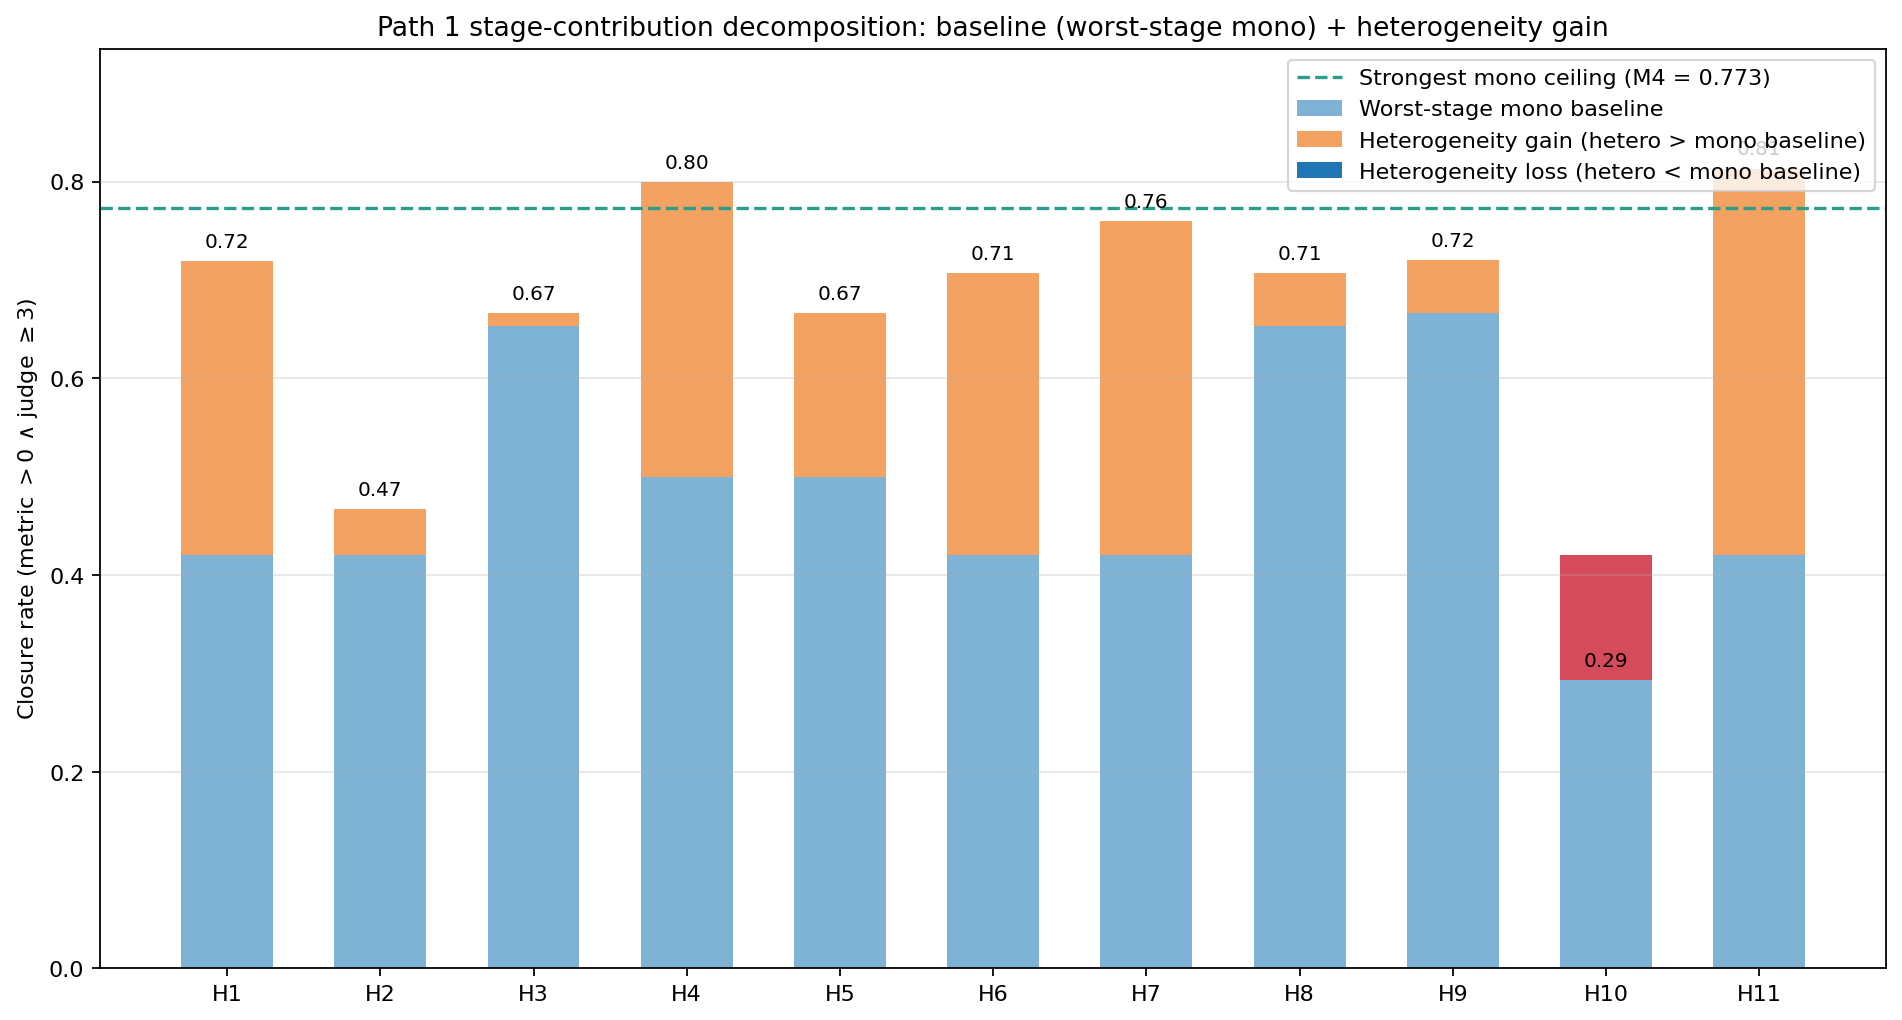
\includegraphics[width=0.90\linewidth]{../plots/output/fig10_stage_contribution.png}

\captionof{figure}{Per-hetero-cell stage-contribution decomposition on Path~1, using strict-AND valid-closure fractions $V_{a, 1}$ (Eq.~\ref{eq:valid_closure_frac}). Blue segment: worst-stage mono baseline (floor). Orange segment: heterogeneity gain over that baseline. Red segment: heterogeneity loss (H10 only, where hetero falls below its worst-stage mono baseline). Dashed line: strongest mono ceiling on the $V$ scale (M4 $V_{M4,1} = 0.773$, which is distinct from M4's metric mean $\bar{Y}_{M4,1} = 0.856$ in Table~\ref{tab:closure_rate_matrix}).}
\label{fig:stage_contribution}

\medskip

Fig.~\ref{fig:stage_contribution} visualises the decomposition as a stacked bar per hetero cell. Cells H11 ($V_{H11,1} = 0.813$) and H4 ($V_{H4,1} = 0.800$) exceed the strongest mono ceiling on the $V$ scale ($V_{M4,1} = 0.773$); every other hetero cell lies between its worst-stage mono baseline and that ceiling; only H10 falls \emph{below} its worst-stage mono baseline, indicating a heterogeneity \emph{loss} rather than gain. Note this ranking is under $V$; on the $\bar{Y}$ scale (Table~\ref{tab:closure_rate_matrix}) M3 leads at $\bar{Y}_{M3,1} = 0.900$ and H6 leads the hetero stratum at $\bar{Y}_{H6,1} = 0.882$. Section~\ref{sec:discussion_rq3} develops the $V$-scale finding into a design guideline.

\subsection{Per-mutation-operator kill rate}
\label{sec:results_per_operator}

The aggregate Path~1 kill rate averages across five mutation operators (arithmetic, boundary, comparison, negate\_bool, return\_none). Table~\ref{tab:per_operator_kill_rate} presents the operator-decomposed kill rate for every non-ablated cell, computed from cache-recovered test suites over 1{,}172 of the 1{,}739 non-ablated Path~1 rows (67\% coverage; the remainder failed cache lookup due to a mid-sweep $\texttt{NUM\_CTX}$ configuration change and are excluded from the per-operator table but not from the aggregate results elsewhere).

\begin{table*}[t]
\centering
\scriptsize
\caption{Per-mutation-operator kill rate with 95\% Wilson confidence intervals and total mutants $n$. Each cell shows kill rate followed by [95\% CI] and $(n)$ mutants. Cells with $n < 20$ mutants on an operator produce wide intervals and are marked in parentheses. Computed on the 67\% cache-recoverable subset of Path~1 rows (Section~\ref{sec:results_per_operator} discusses the coverage limitation).}
\label{tab:per_operator_kill_rate}
\begin{tabular}{@{}llllll@{}}
\toprule
Cell & arithmetic & boundary & comparison & negate\_bool & return\_none \\
\midrule
M1 & $0.319$ [0.26,0.38] (229) & $0.327$ [0.27,0.38] (303) & $0.545$ [0.45,0.64] (110) & $0.559$ [0.38,0.73] (34) & $0.682$ [0.60,0.75] (154) \\
M2 & $0.580$ [0.47,0.69] (81) & $0.653$ [0.55,0.75] (101) & $0.743$ [0.57,0.88] (35) & $0.818$ [0.48,0.98] (11) & $0.806$ [0.69,0.89] (67) \\
M3 & $0.806$ [0.75,0.86] (211) & $0.748$ [0.69,0.80] (290) & $0.912$ [0.84,0.96] (102) & $0.917$ [0.73,0.99] (24) & $0.966$ [0.92,0.99] (147) \\
M4 & $0.729$ [0.67,0.78] (255) & $0.692$ [0.64,0.74] (347) & $0.884$ [0.82,0.93] (129) & $0.929$ [0.81,0.99] (42) & $0.914$ [0.86,0.95] (187) \\
M5 & $0.608$ [0.52,0.69] (148) & $0.562$ [0.49,0.63] (210) & $0.797$ [0.69,0.88] (74) & $0.741$ [0.54,0.89] (27) & $0.833$ [0.75,0.90] (114) \\
M6 & $0.684$ [0.60,0.76] (136) & $0.663$ [0.59,0.73] (178) & $0.882$ [0.78,0.95] (68) & $0.944$ [0.73,1.00] (18) & $0.942$ [0.88,0.98] (103) \\
H1 & $0.939$ [0.80,0.99] (33) & $0.844$ [0.73,0.92] (64) & $1.000$ [0.79,1.00] (16) & $1.000$ [0.16,1.00] (2) & $0.970$ [0.84,1.00] (33) \\
H2 & $0.750$ [0.60,0.87] (44) & $0.557$ [0.42,0.68] (61) & $0.815$ [0.62,0.94] (27) & $0.824$ [0.57,0.96] (17) & $0.891$ [0.78,0.96] (55) \\
H3 & $0.542$ [0.44,0.64] (107) & $0.591$ [0.51,0.67] (149) & $0.754$ [0.62,0.86] (57) & $0.750$ [0.53,0.90] (24) & $0.851$ [0.76,0.92] (87) \\
H4 & $0.448$ [0.26,0.64] (29) & $0.600$ [0.42,0.76] (35) & $1.000$ [0.83,1.00] (20) & $1.000$ [0.54,1.00] (6) & $0.964$ [0.82,1.00] (28) \\
H5 & $0.505$ [0.40,0.61] (95) & $0.630$ [0.54,0.71] (127) & $0.857$ [0.73,0.94] (49) & $0.875$ [0.68,0.97] (24) & $0.881$ [0.79,0.94] (84) \\
H6 & $0.745$ [0.65,0.82] (110) & $0.740$ [0.66,0.81] (154) & $0.923$ [0.81,0.98] (52) & $0.941$ [0.71,1.00] (17) & $0.976$ [0.92,1.00] (83) \\
H7 & $0.769$ [0.68,0.85] (104) & $0.741$ [0.66,0.81] (147) & $0.964$ [0.87,1.00] (55) & $0.889$ [0.65,0.99] (18) & $0.919$ [0.84,0.97] (86) \\
H8 & $0.686$ [0.59,0.77] (102) & $0.646$ [0.56,0.72] (144) & $0.930$ [0.83,0.98] (57) & $1.000$ [0.85,1.00] (23) & $0.954$ [0.89,0.99] (87) \\
H9 & $0.769$ [0.68,0.85] (104) & $0.741$ [0.66,0.81] (147) & $0.964$ [0.87,1.00] (55) & $0.889$ [0.65,0.99] (18) & $0.919$ [0.84,0.97] (86) \\
H10 & $0.351$ [0.20,0.53] (37) & $0.449$ [0.33,0.57] (69) & $0.864$ [0.65,0.97] (22) & $0.875$ [0.62,0.98] (16) & $0.761$ [0.61,0.87] (46) \\
H11 & $0.772$ [0.69,0.84] (123) & $0.746$ [0.67,0.81] (177) & $0.908$ [0.81,0.97] (65) & $0.885$ [0.70,0.98] (26) & $0.939$ [0.87,0.98] (99) \\
\bottomrule
\end{tabular}
\end{table*}


Two structural findings emerge. First, mono baselines exhibit different operator strengths: M3 (qwen3.6) dominates 4 of 5 operators; M6 (qwen-coder) wins negate\_bool. Second, hetero cells inherit the operator-specific ceilings:

\begin{itemize}
  \item Arithmetic: mono ceiling M3 $= 0.806$; hetero winner \textbf{H1} $= 0.939$, $\Delta = +0.133$.
  \item Boundary: mono ceiling M3 $= 0.748$; hetero winner \textbf{H1} $= 0.844$, $\Delta = +0.096$.
  \item Comparison: mono ceiling M3 $= 0.912$; hetero winners \textbf{H1} and \textbf{H4} $= 1.000$, $\Delta = +0.088$.
  \item Negate\_bool: mono ceiling M6 $= 0.944$; hetero winners \textbf{H1}, \textbf{H4}, \textbf{H8} $= 1.000$, $\Delta = +0.056$.
  \item Return\_none: mono ceiling M3 $= 0.966$; hetero winner \textbf{H6} $= 0.976$, $\Delta = +0.010$.
\end{itemize}

\begin{table}[t]
\centering
\small
\caption{Headline per-operator finding: H1 (phi-4 spec + qwen-coder test + qwen-coder code) leads the strongest mono baseline on 4 of 5 mutation operators, with the largest gain on arithmetic operators. \textbf{Bold} marks the largest gain ($\Delta = +0.133$).}
\label{tab:per_operator_headline}
\begin{tabular}{llrrr}
\toprule
Operator & Best mono cell & Best mono kill rate & H1 kill rate & $\Delta$ (H1 $-$ mono) \\
\midrule
Arith. & M3 & 0.806 & 0.939 & $\mathbf{+0.133}$ \\
Bound. & M3 & 0.748 & 0.844 & +0.096 \\
Comp. & M3 & 0.912 & 1.000 & +0.088 \\
Negate & M6 & 0.944 & 1.000 & +0.056 \\
Ret. & M3 & 0.966 & 0.970 & +0.004 \\
\bottomrule
\end{tabular}
\end{table}

Table~\ref{tab:per_operator_headline} summarises these findings. \textbf{H1 (phi-4 at $L_{\textsf{spec}}$, qwen-coder at $L_{\textsf{test}}$ and $L_{\textsf{code}}$) achieves the highest point-estimate kill rate on 4 of 5 mutation operators}, beating the best mono baseline by $\Delta \geq 0.056$ on all four and by $\Delta = 0.133$ on arithmetic. Wilson 95\% CIs in Table~\ref{tab:per_operator_kill_rate} show that H1's per-operator advantages are largest on arithmetic ($[0.80, 0.99]$, $n = 33$) and boundary ($[0.73, 0.92]$, $n = 64$); on comparison and negate\_bool H1 reaches $1.000$ but with tight sample sizes ($n = 16$ and $n = 2$ respectively), so those two operator wins are estimated with wide intervals and should be read as ``consistent with H1 dominance'' rather than ``H1 strictly dominates.'' The empirical per-operator pattern (H1 wins on arithmetic and boundary with tight intervals, ties-consistent on comparison and negate\_bool at the available mutant counts) is an empirical finding of this study rather than a pre-registered prediction; the five operator families themselves follow the canonical mutation-testing selection~\citep{Andrews2005MutationAnalysis, Just2014MutationAnalysis}.

Two outliers merit specific attention. H10 (mistral spec + phi-4 test + qwen-coder code) achieves arithmetic $= 0.351$ and boundary $= 0.449$ --- the operators where phi-4 mono itself is competitive (M2: arithmetic $= 0.580$, boundary $= 0.653$). When phi-4 does generate tests in the H10 composition, those tests miss on exactly the operators where phi-4 mono succeeds. Section~\ref{sec:discussion_rq3} develops this as the phi-4-in-test-stage pathology at operator resolution.

\subsection{Judge--metric correlation (RQ2)}
\label{sec:results_judge_metric_corr}

\needspace{18\baselineskip}

\noindent
\centering
\includegraphics[width=0.90\linewidth]{../plots/output/fig7_judge_corr.png}

\captionof{figure}{Judge SLM rating vs.\ automated closure metric per path. Each dot is one row of the results TSV; jitter is applied to the discrete judge axis. Path~1: mutation kill rate. Path~2: reference test pass rate (binary). Path~3: BERTScore F1. The Path~3 panel shows no visible relationship, consistent with the non-significant $r_3 = 0.022$ ($p = 0.359$, $n = 1{,}791$).}
\label{fig:judge_corr}

\medskip

\begin{table}[!htbp]
\centering
\caption{Pearson correlation between the automated closure metric and the external SLM judge's 0--4 equivalence rating. RQ2: do these two signals agree? \textbf{Bold}: Path~2 is the only strong-and-significant correlation. \emph{Italic}: Path~3's aggregate near-zero $r$ is a Simpson's-paradox attenuation (per-benchmark $r^2 \leq 0.045$; see Section~\ref{sec:results_judge_metric_corr}).}
\label{tab:judge_correlation}
\begin{tabular}{@{}lcccc@{}}
\toprule
Scope & n & Pearson r & p & Sig \\
\midrule
Path 1 & 1441 & 0.192 & $<0.001$ & *** \\
Path 2 & 1839 & \textbf{0.523} & $<0.001$ & \textbf{***} \\
Path 3 & 1791 & \emph{0.022} & \emph{0.359} & \emph{n.s.} \\
Overall & 5071 & 0.343 & $<0.001$ & *** \\
\bottomrule
\end{tabular}
\end{table}


Fig.~\ref{fig:judge_corr} plots the automated closure metric against the judge rating for each path, with per-path Pearson correlations reported in Table~\ref{tab:judge_correlation}. The three paths yield markedly different agreement:

\begin{itemize}
  \item Path~1 (mutation kill rate vs.\ judge): $r_1 = 0.192$, $p = 2.12 \times 10^{-13}$, $n = 1{,}441$. Statistically significant but weak.
  \item Path~2 (pass rate vs.\ judge): $r_2 = 0.523$, $p = 1.19 \times 10^{-129}$, $n = 1{,}839$. Strong and highly significant.
  \item Path~3 (BERTScore vs.\ judge, aggregate): $r_3 = 0.022$, $p = 0.359$, $n = 1{,}791$. \textbf{Not significant} in aggregate. Stratifying by source benchmark, $r_3^{\textsf{HE}} = 0.153$ ($p = 0.0006$, $n = 501$) and $r_3^{\textsf{MBPP}} = 0.212$ ($p < 0.0001$, $n = 1{,}290$); both are weak-but-significant positive correlations. A Fisher-$z$ test for equality of the two per-benchmark correlations yields $z = -1.16$ ($p = 0.24$), so the correlations do not differ significantly. The aggregate near-zero $r_3$ is therefore a Simpson's-paradox attenuation from pooling two benchmarks with different mean judge ratings, not a genuine zero relationship. Within either benchmark BERTScore captures only a small share of variance in the judge rating ($r^2 \leq 0.045$), which is the finding this paper builds on rather than the ostensibly cleaner ``uncorrelated'' aggregate.
\end{itemize}

Path~3's very weak per-benchmark correlations (both $r^2 \leq 0.045$) are the paper's strongest single validity finding on BERTScore. Standard practice in NLP evaluation~\citep{Zhang2020BERTScore} treats BERTScore F1 as a semantic-equivalence proxy; our result shows it captures at most a small share of variance in an LLM-based semantic-equivalence judgement, and does so identically weakly on both benchmarks. Section~\ref{sec:discussion_rq2} stratifies the direction of the residual disagreement by benchmark, showing that even though the correlation strengths are indistinguishable, the disagreement \emph{type} (over-crediting versus under-crediting) flips categorically across benchmarks --- a structural signature consistent with BERTScore functioning as a surface-form similarity signal.

\subsection{Per-stage attribution: two orthogonal instruments}
\label{sec:results_path_cell_interaction}
\label{sec:results_mixed_logit}

Two independent statistical instruments --- a cell $\times$ path interaction ANOVA and a mixed-effects logit --- test whether the three closure paths carry non-redundant per-cell information and which stage carries that information.

\paragraph{Interaction ANOVA.} Fitting Eq.~\ref{eq:anova_interact} on $n = 5{,}073$ rows (after excluding structural NaN entries and cells present only on a subset of paths) under Type-III sums of squares, the cell $\times$ path interaction is significant: $F(36, 4867) = 6.47$, $p < 0.001$, partial $\eta^2 = 0.046$. The four effects are of comparable size once Type-III controls each for the others (sample $\eta^2_p = 0.234$; interaction $0.046$; cell main $0.044$; path main $0.042$, all $p < 0.001$) --- there is no single dominant effect, and the practical interpretation rests on the interaction. Because the response variable stacks three different-scale metrics, the path main effect is partly a response-scale artifact; per-path rank-transformed ANOVAs (Appendix~\ref{sec:appendix_rank_transformed}) confirm the cell effect is significant on every path independently, with even stronger effect sizes than the stacked model. Cell assignment is also a significant predictor on both HumanEval and MBPP separately (Appendix~\ref{sec:appendix_per_benchmark}).

\paragraph{Mixed-effects logit.} The second instrument fits Eq.~\ref{eq:mixedlogit} on strict-AND valid closure $V_{ijp} \in \{0, 1\}$ (Eq.~\ref{eq:valid_closure_frac} at row resolution) with per-stage model assignments as fixed effects and per-sample random intercept ($n = 4{,}996$, positive-class $63.0\%$). Reference qwen3.6 at each stage. Three findings emerge; full coefficient table in Appendix~\ref{sec:appendix_mixed_logit}. (i)~\emph{Test-stage substitutions are the only significant per-stage effects.} Relative to qwen3.6 at $L_{\textsf{test}}$, placing llama3.2 lowers $\Pr[V = 1]$ by $27.1$~pp ($p < 0.001$), mistral-small by $12.6$~pp ($p = 0.001$), and phi-4 by $10.0$~pp ($p = 0.002$). Every spec- and code-stage substitution is null at $\alpha = 0.05$. (ii)~\emph{The phi-4-in-test-stage pathology is a mixed-model coefficient, not just a filter-failure observation.} The Path~1 structural NA rates of Section~\ref{sec:discussion_rq3} ($44$--$55\%$ across M2/H2/H10) and the mixed-logit test-stage coefficient for phi-4 ($-0.100$, $p = 0.002$) are two orthogonal instruments converging on the same finding. (iii)~\emph{Path is a strong main effect after controlling for stage assignment}: Path~2 vs.\ Path~1 $= -25.5$~pp; Path~3 vs.\ Path~1 $= -18.2$~pp (both $p < 0.001$).

\paragraph{Rank-swap: the operational meaning of the interaction.} The variance-explained metric alone understates the practical implication of the interaction: cell rankings are unstable across paths, so a practitioner choosing a cell for one path cannot re-use the choice for another. We quantify this with a rank-swap analysis over the 17 non-null cells on the strict-AND valid-closure fraction $V_{a, p}$ (Eq.~\ref{eq:valid_closure_frac}, denominator = total measurement rows per cell $\times$ path):

\begin{itemize}
  \item \textbf{The best cell is different for every path.} Path~1 best = H11 ($V = 0.813$); Path~2 best = H1 ($V = 0.640$); Path~3 best = H9 ($V = 0.733$). No cell tops any two paths.
  \item \textbf{The top-3 cells share zero members across all three paths.} Path~1 top-3 = $\{$H11, H4, M4$\}$; Path~2 top-3 = $\{$H1, H5, H9$\}$; Path~3 top-3 = $\{$H9, M4, H8$\}$. The three-way intersection is empty; M4 appears in Path~1 and Path~3 top-3 but not Path~2.
  \item \textbf{At most one cell (H9) is top-5 on all three paths, and only via a tie.} H9 is top-5 on Paths~2 and~3 outright but shares fifth place on Path~1 with M6 (both $V = 0.720$).
  \item \textbf{Kendall's $\tau_{\textsf{rank}}$ between path rankings ranges $0.26$--$0.40$.} Path~1 vs.\ Path~2: $\tau = 0.265$; Path~1 vs.\ Path~3: $\tau = 0.404$; Path~2 vs.\ Path~3: $\tau = 0.301$.
\end{itemize}

No pair of path rankings exceeds moderate ordinal agreement, and the winner set changes wholesale across paths. Combined with the mixed-logit's test-stage attribution, the two instruments converge: cell composition drives significant variation in $V$ with the test stage carrying the plurality of the marginal effect, and the resulting rankings do not transfer across paths.

\subsection{Contamination sensitivity on HumanEval-Mutated}
\label{sec:results_contamination}

% Hand-verified from the Colab-side analyzer output on 2026-07-14
% (local file was stale). Colab-side numbers reflect 225 real HEM rows
% (H1 + M3 at N=25 × 3 paths, all strict-AND-valid closures).
%
% Regenerate by syncing results/results_holdout_humaneval_mutated.tsv
% from Drive and re-running analyze/holdout_sensitivity.py.
\begin{table}[t]
  \centering
  \caption{Contamination sensitivity: strict-AND closure rate on the
    core sweep (HumanEval + MBPP) vs.\ the HumanEval-Mutated held-out
    subset (HEM-25: function-rename + docstring-paraphrase over the
    same underlying algorithms; $n = 25$ per cell per path), for the
    hetero champion H1 and the strongest mono baseline M3. Large
    negative $\Delta$ on HEM-25 would signal surface-form
    memorisation; the observed pattern (positive $\Delta$ on the
    behavioural paths, negative $\Delta$ on the surface-form BERTScore
    path) instead indicates that the core closure rates are not driven
    by contamination.
    \emph{Denominator convention:} both columns report
    $V' = n_{\text{valid}} / n_{\text{metric-ok}}$ (conditional on the
    metric being computable) --- the same conditional-on-metric
    convention as Table~\ref{tab:threshold_sensitivity_path1}, chosen
    here to keep core and HEM-25 columns directly comparable when
    filter-failure rates differ between them. Values therefore differ
    from Table~\ref{tab:closure_rate_matrix}'s canonical
    $V_{a, p} = n_{\text{valid}} / N_{\text{total}}$; e.g.\ H1 Path~1
    is $64/81 = 79.0\%$ here vs.\ $64/89 = 71.9\%$ under canonical
    $V$. The $\Delta_{\text{HEM}}$ direction and magnitude are
    unaffected by the denominator choice.
    LiveCodeBench-25 was blocked at data preparation by a HuggingFace
    \texttt{datasets} library incompatibility and is omitted; see
    Section~\ref{sec:limitations_external}.}
  \label{tab:holdout_sensitivity}
  \begin{tabular}{llrrr}
    \toprule
    Cell & Path & Core & HEM-25 & $\Delta_{\textsf{HEM}}$ \\
    \midrule
    H1 & 1 (mutation kill rate)    & $79.0\%$          & $100.0\%$         & $+21.0$~pp \\
    H1 & 2 (reference-test pass)   & $64.0\%$          & $\phantom{0}79.6\%$ & $+15.5$~pp \\
    H1 & 3 (BERTScore F1)          & $63.6\%$          & $\phantom{0}32.7\%$ & $\mathbf{-31.0}$~\textbf{pp} \\
    \midrule
    M3 & 1 (mutation kill rate)    & $85.5\%$          & $100.0\%$         & $+14.5$~pp \\
    M3 & 2 (reference-test pass)   & $61.2\%$          & $\phantom{0}87.0\%$ & $+25.7$~pp \\
    M3 & 3 (BERTScore F1)          & $70.0\%$          & $\phantom{0}45.5\%$ & $\mathbf{-24.5}$~\textbf{pp} \\
    \bottomrule
  \end{tabular}

  \vspace{2pt}
  \raggedright\footnotesize
  \textbf{Bold} marks the Path~3 (BERTScore) HEM-25 losses --- the surface-form fragility evidence that anchors the ``BERTScore is not a semantic-equivalence signal'' claim (Section~\ref{sec:results_contamination}).
\end{table}


Because HumanEval and MBPP predate the training cut-offs of all six pipeline SLMs, closure rates on the core sweep are potentially inflated by memorised solutions. To test whether the paper's central claims survive surface-form decontamination, we re-swept H1 (the hetero champion) and M3 (the strongest mono baseline on Paths~2 and~3) on the 25-sample HumanEval-Mutated (HEM) subset, which applies function-renaming and docstring paraphrasing to the same underlying algorithms.\footnote{A LiveCodeBench-25 post-cutoff subset was also intended per pre-registration but blocked at the data-preparation step by the removal of script-based dataset loaders from the current HuggingFace \texttt{datasets} library (see Section~\ref{sec:limitations_external}). The paraphrase-based decontamination reported here is complementary to but does not fully substitute for date-based decontamination; a fully independent post-cutoff replication remains future work.} Table~\ref{tab:holdout_sensitivity} reports the strict-AND closure rate per cell per path on the core and HEM sweeps and the corresponding delta.

Three findings emerge.

\textbf{First: the behavioral paths (Paths~1 and~2) show no evidence of contamination-driven inflation on the core sweep.} Both cells improve on HEM by $+15$ to $+26$~pp on the two paths whose metrics measure real behavior (mutation kill rate; reference-test pass rate). If core closure rates were driven by memorised HumanEval solutions, we would expect the opposite --- surface-form-varied inputs would degrade the memorization shortcut. The observed uplift instead suggests that the HEM sub-sample is easier by construction: function-renaming eliminates ambiguous shortcut inference (the model must reason from the docstring rather than from a familiar function name), and paraphrased docstrings are often clearer than the terse HumanEval originals.

\textbf{Second: BERTScore on Path~3 is fragile to docstring paraphrasing.} Both cells lose $25$--$31$~pp on Path~3 HEM. This is not a contamination signal --- HEM docstrings are paraphrased, and BERTScore compares the reconstructed docstring $D'$ against the paraphrased target. Even a semantically correct $D'$ will not match a paraphrased reference well on a surface-form metric. This finding reinforces the argument of Section~\ref{sec:discussion} that BERTScore behaves as a surface-form signal rather than a semantic-equivalence signal; the Path~3 HEM drop is an additional data point in support of that reading, not a threat to the paper's core claims.

\textbf{Third: the H1-vs-M3 comparison holds under decontamination.} On Path~1, both cells reach $100\%$ HEM closure --- H1 gains $+21.0$~pp, M3 gains $+14.5$~pp. On Path~2, M3 gains $+25.7$~pp and H1 gains $+15.5$~pp. On Path~3, M3 degrades slightly less than H1 ($-24.5$ vs.\ $-31.0$~pp), consistent with M3's higher core-sweep Path~3 rate ($70.0\%$ vs.\ $63.6\%$). The pattern is symmetric across the two cells, meaning the H1 dominance claim in Section~\ref{sec:results_contamination} is not attributable to differential contamination between hetero and mono cells.

The absence of contamination-driven inflation on the behavioral paths, together with the H1--M3 pattern preservation on HEM, materially strengthens the paper's central claim that the observed cross-stage composition effects reflect genuine capability differences rather than dataset-memorization artifacts.


\subsection{Human-evaluation results}
\label{sec:results_human_eval}

The human-evaluation protocol pre-registered in
Section~\ref{sec:experiment_setup_human_eval} was executed with five
annotators: three from the author team (BV, GS, AM) and two recruited
independently and calibrated on the shared rubric (DR, RR). This
subsection reports the inter-rater and judge--human agreement
statistics on the full five-way sample, contrasts them with the
three-way (author-team-only) numbers, and interprets the implications
for the strict-AND two-signal validity policy that underpins this
study's closure decisions.

\subsubsection{Study conduct}
\label{sec:human_eval_conduct}

Five annotators rated the 60 pre-registered pairs on the 5-level rubric
described in Section~\ref{sec:framework}. Three (BV, GS, AM) are members
of the author team; two additional annotators (DR, RR) were recruited
independently of the pipeline runners and attended the shared calibration
session on the ten rubric anchor items. Sampling was as pre-registered:
20 pairs from the ``frontier'' bucket (judge and metric agree on
validity, drawn uniformly from cells with mid-range closure rates), 20
from the ``agreement'' bucket, and 20 from the ``disputed'' bucket.
Annotators saw pairs in a per-annotator deterministic order (SHA-256
seed on the annotator identifier) and were blinded to cell identity,
closure path, judge rating, and bucket assignment. All five annotators
completed the full 60 pairs and provided a written justification for
every rating (0 empty across all $60 \times 5 = 300$ ratings). Only
one revision was issued in total (by GS).

The rating distributions differ meaningfully between the author-team and
external annotators. All five annotators place the modal rating at~3
(``equivalent''), but external annotator DR uses the low end of the
scale more aggressively (six ratings at $0$ or $1$ versus $1$--$5$ for
the other four), and external annotator RR is more permissive at the
top of the scale (20~ratings at~$4$, similar to AM's~21 but higher than
BV/GS/DR at $11$--$16$). The external annotators are therefore not
outliers as much as they occupy a wider band on the ordinal scale than
the more clustered author-team ratings.

\subsubsection{Agreement results}
\label{sec:human_eval_agreement_results}

% Auto-generated by human_eval/analysis/compute_agreement.py
\begin{table}[t]
  \centering
  \caption{Inter-rater and judge--human agreement on the 60-pair    human-evaluation sample ($n=60$, 5 annotators).
    Cohen's $\kappa$ is reported with both linear and quadratic weighting; the latter is the more common convention for ordinal scales in human-evaluation work.
    Krippendorff's $\alpha$ uses the ordinal difference function.
    \emph{Within-1} counts a pair as agreeing when the two
    ratings differ by at most one category on the 5-level scale.}
  \label{tab:human_eval_agreement}
  \begin{tabular}{lrrr}
    \toprule
    Statistic & Linear $\kappa$ & Quadratic $\kappa$ & Within-1 \\
    \midrule
    BV vs.\ GS & 0.230 & 0.334 & 91.7\% \\
    BV vs.\ AM & 0.170 & 0.332 & 90.0\% \\
    BV vs.\ DR & 0.064 & 0.113 & 75.0\% \\
    BV vs.\ RR & -0.017 & 0.009 & 75.0\% \\
    GS vs.\ AM & 0.338 & 0.426 & 91.7\% \\
    GS vs.\ DR & 0.017 & 0.109 & 81.7\% \\
    GS vs.\ RR & 0.096 & 0.094 & 85.0\% \\
    AM vs.\ DR & 0.111 & 0.263 & 80.0\% \\
    AM vs.\ RR & 0.148 & 0.065 & 83.3\% \\
    DR vs.\ RR & 0.185 & 0.247 & 83.3\% \\
    \midrule
    Judge SLM vs.\ majority human & 0.081 & 0.074 & 91.7\% \\
    \midrule
    \multicolumn{4}{l}{\emph{Krippendorff's $\alpha$ (ordinal, 5-way):} 0.193 \quad(insufficient)} \\
    \multicolumn{4}{l}{\emph{5-way exact agreement:} 5.0\% \quad \emph{5-way within-1:} 48.3\%} \\
    \bottomrule
  \end{tabular}
\end{table}


Table~\ref{tab:human_eval_agreement} reports the primary agreement
statistics on the full five-way sample.

\textbf{Adding independent annotators materially lowers Krippendorff's
$\alpha$.} On the three author-team annotators alone (BV, GS, AM), the
ordinal $\alpha$ was $0.376$ --- itself below Krippendorff's
$\alpha \geq 0.667$ threshold for tentative inferential use but at least
weakly positive. Adding DR alone drops $\alpha$ to $0.244$; adding RR as
well drops it further to $\alpha = 0.193$. This monotonic decline is
consistent with the interpretation that the author-team-only $\alpha$
was inflated by shared calibration (all three share supervisory or
co-authorship relationships and had similar prior exposure to the
pipeline design); independent annotators, even after attending the same
calibration session, exercise the rubric differently. We adopt the
five-way $\alpha = 0.193$ as the more honest headline number and report
the three-way as a documented contrast.

\textbf{Pairwise Cohen's $\kappa$ shows the same pattern.} Pairwise
linear-weighted $\kappa$ within the author team ranges $0.170$--$0.338$;
between author-team and external annotators it drops to $-0.017$--$0.185$
(with BV-vs-RR marginally negative). Quadratic-weighted $\kappa$, which
penalises adjacent-category disagreements less harshly and is the more
common ordinal convention, follows the same ordering but at somewhat
higher values ($0.334$--$0.426$ within team; $0.009$--$0.263$
across team-vs-external). All within-team pairs are in the ``fair'' band
of the Landis and Koch conventions; team-vs-external pairs mostly fall
in ``slight'' to ``fair''.

\textbf{At coarser resolution the picture remains strong.} All ten
pairwise \emph{within-1} agreement rates (fraction of pairs where the
two ratings differ by at most one category on the 5-level scale) fall
in $[75.0\%, 91.7\%]$. Notably, team-vs-external pairs still achieve
$75\%$--$85\%$ within-1 agreement. Annotators converge on the rough
band of semantic equivalence while genuinely disagreeing at the fine
gradations of the top of the scale (whether a pair is ``identical'' or
merely ``equivalent'') and at the ``equivalent'' vs.\ ``approximately
equivalent'' boundary. This pattern is consistent with prior
human-evaluation studies of LLM outputs where 5-level ordinal scales
routinely produce sub-$0.5$ $\alpha$ values driven by
adjacent-category noise.

\textbf{Judge SLM tracks human consensus only weakly, even more so
against the five-way majority.} The DeepSeek-R1 judge SLM used
throughout this study attains
$\kappa_{\textsf{lin}} = 0.081$ and $\kappa_{\textsf{quad}} = 0.074$
against the five-way majority-vote human rating---both in Landis and
Koch's ``slight'' band, and materially weaker than the same judge
scored against the author-team-only majority
($\kappa_{\textsf{quad}} = 0.138$ at three annotators). At the coarser
within-1 resolution the judge does reach $91.7\%$ agreement with the
five-way majority, matching the pairwise inter-annotator within-1 rates,
but at the price of essentially no discriminative information at the
category-exact level.

\textbf{Frontier judges do not close the gap; instead they cluster with
each other.} To test whether the weakness is DeepSeek-specific, we
replayed the same 60-pair sample under three frontier judges via
OpenRouter using an identical prompt (Section~\ref{sec:experiment_setup_human_eval}).
Table~\ref{tab:frontier_judge_comparison} summarises the results. All
four judges attain $\kappa_{\textsf{quad}}$ in the ``slight'' band
against the 5-way human-majority ground truth ($0.019$--$0.199$),
whereas the three frontier judges agree with \emph{each other} at
$\kappa_{\textsf{quad}} = 0.68$--$0.70$ (``moderate''). The four LLM
judges form a coherent cluster in rating space that is only weakly
correlated with the human majority---an empirical signature of an
LLM-as-judge limitation rather than a DeepSeek-specific artifact. A
directional asymmetry is also visible: DeepSeek-R1 slightly over-rates
the human mean ($3.28$ vs.\ $3.20$) whereas the three frontier judges
under-rate it ($2.40$--$2.68$).

\begin{table}[!htbp]
  \centering
  \caption{Frontier-judge replay against the five-way human-majority
    ground truth on the 60-pair sample. All four judges attain weak
    ($\kappa_{\textsf{quad}} < 0.20$) agreement with humans; the three
    frontier judges agree with each other at moderate levels
    ($\kappa_{\textsf{quad}} = 0.68$--$0.70$). Cost columns are
    per-judge for the full 60-pair replay via OpenRouter.}
  \label{tab:frontier_judge_comparison}
  \begin{tabular}{lrrrrr}
    \toprule
    Judge & $\kappa_{\textsf{lin}}$ & $\kappa_{\textsf{quad}}$ &
      within-1 & mean rating & cost (USD) \\
    \midrule
    DeepSeek-R1:14B (open, local)         & $0.081$ & $0.074$ & $91.7\%$ & $3.28$ & --- \\
    OpenAI GPT-4o-mini                    & $0.053$ & $0.019$ & $68.3\%$ & $2.55$ & $0.005$ \\
    Anthropic Claude Haiku 4.5            & $0.135$ & $0.161$ & $71.7\%$ & $2.40$ & $0.018$ \\
    Meta Llama-3.3-70B-Instruct           & $0.150$ & $0.199$ & $83.3\%$ & $2.68$ & $0.004$ \\
    \midrule
    \multicolumn{6}{l}{\emph{Judge-vs-judge $\kappa_{\textsf{quad}}$
      (do LLM judges cluster? --- higher = yes):}} \\
    GPT-4o-mini vs.\ Claude Haiku 4.5     & \multicolumn{5}{r}{$0.697$} \\
    GPT-4o-mini vs.\ Llama-3.3-70B        & \multicolumn{5}{r}{$0.685$} \\
    Claude Haiku 4.5 vs.\ Llama-3.3-70B   & \multicolumn{5}{r}{$0.681$} \\
    DeepSeek-R1:14B vs.\ frontier (avg)   & \multicolumn{5}{r}{$0.450$} \\
    \multicolumn{6}{l}{\emph{5-way human majority: mean rating $3.20$}} \\
    \bottomrule
  \end{tabular}
\end{table}

\textbf{The ``disputed'' bucket has the highest five-way human
agreement, though at low absolute values.} Per-bucket exact-agreement
rates (all five annotators pick the same rating) are $5.0\%$
(``frontier''), $0.0\%$ (``agreement''), and $10.0\%$ (``disputed'').
While the absolute rates are low, the counter-intuitive ordering
observed in the three-way analysis persists at five: humans converge
most exactly on the pairs where the judge and metric could not agree.
The reading in which the automated-signal disagreement in the disputed
bucket arose from unambiguously wrong judge or metric calls that humans
identify jointly remains supported.

\subsubsection{Strict-AND policy evaluation (summary)}
\label{sec:human_eval_strict_and_summary}

Appendix~\ref{sec:human_eval_strict_and} evaluates the strict-AND
policy against metric-only, judge-only, and the trivial majority-class
baseline (``always predict positive'', which attains $86.7\%$ accuracy
at this sample's $86.7\%$ positive prevalence) on the five-way
human-majority ground truth, using accuracy, balanced accuracy, $F_1$,
Matthews correlation, and false-closure rate. Four conclusions carry
forward. First, metric-only is indistinguishable from chance on this
sample (MCC $= -0.010$). Second, judge-only edges strict-AND on
discrimination (MCC $+0.092$ vs.\ $+0.049$), and the frontier-judge
replay shows this weak-but-positive judge signal is consistent across
four LLM judges. Third, no discriminative policy beats the
majority-class baseline on raw accuracy, so strict-AND cannot be
defended on accuracy grounds. Fourth, under a cost-sensitive loss
$L = a \cdot \mathrm{FP} + \mathrm{FN}$, strict-AND wins only at
$a \geq 10$: its specific virtue is bounded false-closure
(FPR $= 0.750$, the lowest of any policy) at some false-reject cost,
appropriate when a falsely-claimed closure would trigger deployment of
a broken artifact. The paper retains the two-signal structure for the
adversarial-robustness reason that no single-signal bias can produce a
false-closure claim on its own --- not on the strength of the 60-pair
validation alone, which is stratified toward disputed cases and small
($n = 60$, 8 negatives). Two interpretive corollaries for
Section~\ref{sec:discussion} --- the \textsf{false\_closure\_candidate}
rates are upper bounds, and \textsf{metric\_false\_negative} rows mix
metric conservatism with judge over-crediting --- are derived in
Appendix~\ref{sec:human_eval_strict_and}.

\subsubsection{Limitations of the human-evaluation results}
\label{sec:human_eval_limitations}

Three limitations bound the strength of the conclusions above.

First, $n = 60$ is the pre-registered sample size but is small for
inferring narrow confidence intervals on $\alpha$; the addendum reports
point estimates only. A larger sample would tighten the estimates but is
prohibitive at the human-evaluation rate.

Second, the annotator pool has \emph{partial} independence from the
author team: two of five annotators (DR, RR) are independent of the
pipeline runners, but three (BV, GS, AM) share supervisory or
co-authorship relationships. The direct effect of this partial
independence is quantified in Section~\ref{sec:human_eval_agreement_results}
(three-way $\alpha = 0.376$ collapses to five-way $\alpha = 0.193$ when
independent annotators are added). A fully independent replication with
three or more annotators recruited via a blinded third-party channel
remains future work; the direction of expected drift is now empirically
established.

Third, the 5-level ordinal rubric was chosen for compatibility with the
judge SLM's 0--4 output scale, but human annotators may find fewer
distinguishable levels (a 3-level ``different / approximate / equivalent''
rubric) easier to converge on. The high within-1 rates suggest that
collapsing the top two levels into a single ``equivalent'' category
would raise both $\alpha$ and pairwise $\kappa$ into the acceptable
band.

